\chapter{Implementation}\label{ch:impl}

\todo[inline]{Generally: don't make this section too long I'd say!}

After laying out the theoretical foundations of detecting missing method calls using the majority rule in the last chapter, this chapter focusses on the practical side and on the internal workings of the system we developed.
It explains the steps from receiving the input program to outputting a list of anomalies which hint at potentially missing method calls.
We give details about design decisions taken and the reasoning behind them, pitfalls that had to be overcome and the trade-offs that had to be accepted.
Additionally, we explore some of the mistakes made and dead ends that we encountered.

\section{Overview}

Our system is (primarily) a system for detecting missing method calls.
It works by statically analyzing a given software application, extracting the type usages which it contains and finally determining if any of them are anomalous by the Majority rule as described in Section \ref{sec:majority}.
The end result should be a list of locations which are potentially missing a method call.
Given a software system, which shall be tested for anomalies, conceptually the following steps have to be realized:

\begin{enumerate}
    \item Extract all type usages from the software
    \item For each type usage $x$ among them:
    \begin{enumerate}
        \item Search for type usages which are exactly similar to $x$ (i.e. calculate $E(x)$)
        \item Search for type usages which are almost similar to $x$ (that is determine $A(x)$)
        \item Calculate the strangeness score of $x$
        \item Extract the list of potentially missing calls and their likelihood $\phi$
    \end{enumerate}
    \item Output a list of anomalous type usages, sorted by their $\operatorname{S-score}$, together with the calls they are potentially missing
\end{enumerate}

\begin{figure}[h]
\centering
\begin{tikzpicture}
    \tikzset{vertex/.style={draw,rounded corners,align=center}}
    \tikzset{edge/.style = {->,> = latex'}}

    % start dot
    \node[fill=white] (startTxt) {Application};
    \node[fill=black,circle,inner sep=2pt] (start) [below = 0.25cm of startTxt] {};

    % java + db
    \node[vertex] (j1) [right = 1.5cm of start] {Read\\bytecode};
    \node[vertex] (j2) [right = 0.5cm of j1] {Extract\\type usages};
    \node[vertex] (db1) [right = 0.5cm of j2] {Persist\\type usages};

    \draw[edge] (start) to (j1);
    \draw[edge] (j1) to (j2);
    \draw[edge] (j2) to (db1);

    % py + db + end
    \node[vertex] (db2) [below = 0.25cm of db1] {Answer\\query};
    \node[vertex] (py1) [below left = 0.5cm of db2] {Request\\current set};
    \node[vertex] (py2) [below right = 0.5cm of db2] {Calculate\\ $\operatorname{S-score}$};
    \node[fill=black,circle,inner sep=2pt] (end) [right = 1.5cm of py2] {};
    \node[fill=white,align=center] (endTxt) [above = 0.25cm of end] {List of\\anomalies};

    \draw[edge] (py1) to (db2);
    \draw[edge] (db2) to (py2);
    \draw[edge] (py2) to (end);

    % big dashed boxes
    \node[label=above left:{Java}, draw=black, thick, dashed, inner sep=0.25em, fit=(j1) (j2)] {};
    \node[label=right:{Database}, draw=black, thick, dashed, inner sep=0.25em, fit=(db1) (db2)] {};
    \node[label=left:{Python}, draw=black, thick, dashed, inner sep=0.25em, fit=(py1) (py2)] {};

\end{tikzpicture}
\caption{System overview}
\label{fig:overview}
\end{figure}
\todo{make a bit nicer (alles bisi auseinander ziehen?), better position dash box labels | POTENTIALLY add the retrieve sets step to python?}
% https://tex.stackexchange.com/questions/58878/tikz-set-node-label-position-more-precisely

%-- description of system
However, this simple outline does not represent the actual realities of the system.
Instead of a singular process with [flat / not branching / \ldots] flow, it is split into three different parts which are laid out in Figure \ref{fig:overview}.
First, a java application reads the byte code of the program under analysis and iterates over all method definitions to extract the type usages which are present.
The extracted type usages are then persisted in a database to ensure flexibility and high performance in the following analysis phase.
For the actual anomaly detection we use a relatively simple python program to enable fast prototyping and again flexibility.
It goes through all sets of type usages (more on those sets in Section \ref{sec:anomaly}), requests the type usages in the set and calculates their strangeness score.
\todo{partitions instead of sets?}
After iterating through all the sets of the application it finally outputs the results.

%summary of rest
The following sections give a more in depth explanation of the separate steps.
\todo{smth more?}

\section{Bytecode Analysis}\label{sec:bytecode}
\todo[inline]{maybe rename section?}

%-- general intro
We use Soot \footnote{\url{https://sable.github.io/soot/}} for the bytecode analysis.
Soot was originally a Java optimization framework but has since evolved to support a wide range of usages.
One can use it to analyse, instrument, optimize and visualize Java and Android applications.
For this purpose it provides call graph construction, points-to analysis, def or use chains, inter and intra-procedural data-flow analysis and taint analysis.
We do not need most of it's functionality, but simply use it to statically extract type usages from the input application.

%-- why bytecode over sourcecode
It would be possible to extract type usages from the source code, but extracting them from compiled code has some advantages.
The JVM byte code is very standardized and so is the Dalvik byte code found in Android applications, which facilitates the analysis.
While Soot supports source code analysis in theory, it only works up to Java 7 and byte code analysis is the recommended approach.
Besides that, using compiled applications simplifies our experimental setup and as a marginally useful side-effect, it also helps with analyzing obfuscated applications.
Finally, there are no real disadvantages to this approach, if the program is only available as source code we can simply compile it before analyzing it.

%-- some more in depth info on how soot does what it does?
Soot operates by transforming the given program into intermediate representations which can then be optimized or analysed.
It provides four intermediate representations with different use cases, we use Jimple, Soot's primary representation.
Jimple is a typed 3-address representation, which is especially suited for optimization, but also suffices for our purpose.

%-- soot startup and settings?
Soot is a very powerful framework and one can customize it to carter quite specialized requirements.
We will mostly analyze Android applications and the settings we are using reflect this.
In Figure \ref{fig:sootparam} we have listed the most important settings we are using to configure Soot.

\todo[inline]{more detailed description of settings? i think not}

\begin{figure}[t]
    \centering
    \begin{tabular}[h]{c|c|c}
    Option & Parameter & Explanation \\ \hline
    \code{-app } & - & Run in application mode \\ \hline
    \code{-keep-line-number} & - & Keep line number tables \\ \hline
    \code{-output-format} & none & Set output format for Soot \\ \hline
    \code{-allow-phantom-refs } & - & Allow unresolved classes \\ \hline
    \code{-src-prec} & apk-class-jimple & Sets source precedence to format files \\ \hline
    \code{-process-multiple-dex} & - & Process all DEX files found in APK \\ \hline
    \code{-android-jars} & [path] & The path for finding the android.jar file \\ \hline
    \end{tabular}
    \caption{The parameters passed to Soot}
    \label{fig:sootparam}
\end{figure}

\section{Extracting Type Usages}

\todo[inline]{
some more on extraction! + the algorithm!
some information on what kind of further analysis is attempted (local must alias, bla)
general / not sure where yet: 
explain the changes I made to their code ie proper refactoring, etc
}

%-- general ablauf
The Soot execution is divided into a number of 'phases' each of which has a specific task like for example the aggregation of local variables.
The actual work is done by so called transformations, which are able to modify the input they receive but are not required to do so.
The phases are further grouped into 'packs' and the registered packs are applied successively during the execution.
We register a custom piece of code in the Jimple transformation pack, which is applied to every method in the analysed program.

%--- what is the transformer doing?
This custom transformation receives as input a Jimple representation of the method body it is currently analyzing.
To extract the type usages, it iterates through all the statements in the method and marks those which are invoking a method.
In the end it has extracted a list of all method calls that are happening in this method.
It now iterates through this list of method calls and groups them into type usages.
To do so, it first checks on which variable or object the current call was invoked and checks if there is already a type usage for this object.
If there is, it adds the call to the type usage and advances to the next method call in the list.
If there is no type usage for the object so far, it creates a new one.
After completing this process for all method invocations in the method body the analysis is complete and it returns the list of type usages it extracted.

%-- local must alias analysis
One important step of this analysis is the 'LocalMustAliasAnalysis', which attempts to determine if two local variables (at potentially different program points) must point to the same object.
This is necessary to decide if the calls made on these locals should be grouped into one type usage.
The underlying abstraction is based on global variable numbering and follows the ideas presented by Lapowsky et al. \cite{lapkowski1998extended} with some minor adaptions.
This analysis is a Soot feature and in test runs on big applications we noticed that it can be very expensive.
Because of this we made it optional, however for our benchmarks and evaluation we were able to use it.

%-- ignoring some classes
One additional detail is that we are excluding some classes from the Android analysis for performance reasons.
The packages we exclude in this manner are \code{java.*}, \code{android.*}, \code{soot.*} and  \code{javax.*}.
These are all framework classes and we are primarily interested in the type usages occurring in the application itself not in the framework.
This means that we do not store type usages that occur \emph{inside} of those classes, we do, however, still record usages of them.
\todo[inline]{
explain a bit better that these classes are kind of exactly what we are most interested in as far as type usages go, but we don't want too step ITNO them
+ make sure this works good together with coresponding paragraph in the next section
}
\todo{some changes that had to be made to the analysis framework for android analysis?}

\section{Storing Type Usages}

%intro / übergang + general info
After the transformer has analyzed the current method body and extracted a list of type usages from it, we persist them into a database.
For this, we are using HSQLDB\footnote{\url{http://hsqldb.org/}}, a SQL relational database written in Java, which provides a multithreaded and transactional database engine with in memory or disk based tables.
We chose HSQLDB because it is small and has good performance as well as an easy setup.
Additional arguments where its permissive license and the large number of features it supports.

%- why are we using a database at all?
In their work, Monperrus et al. save all data in a text based format, but this means they need to parse everything again for the analysis, which can be slow and require a lot of memory for large inputs.
Additionally, the data takes up a lot of storage space when persisted to disk.
In contrast, using a database has many positive ramifications.
First off, retrieving data from a database is fast and we can access the data selectively based on changing criteria.
Additionally, we gain a lot of flexibility and it becomes easier to extend both, the stored data and the analysis itself.
(This enables us to quickly build several prototypes of the analysis using Python.))

% --- continue writeout here ---
% what we really wanna do: build big database collecting ALL tus -> better analysis
its already useful to analyze one application in separation
but we really care about the framework / library classes which are used by more than one application
analyze a lot of applications using the same framework/library
on these classes we can build a large dataset of type usages -> have much more information to determine if a tu is an anomaly or not
-> having a database really helps with that (can hold a lot of data + can selectively query it are the main points i think?)
of course it's useful to ALSO analyse tus over classes which are private to my application (if there is enough data)
    but the framework thing is just a) easier to get the info and b) kind the point of this thingy?

\begin{figure}[h]
    \centering
    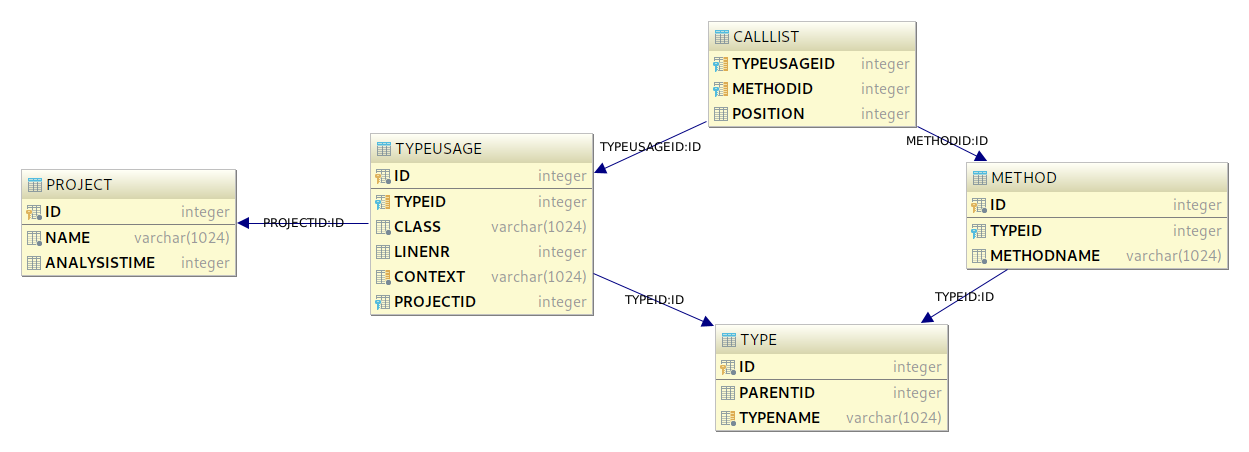
\includegraphics[width=\textwidth]{figures/database_layout-light}
    \caption{Overview of Database Tables}
    \label{fig:db_layout}
\end{figure}
\todo[inline]{
    REMOVE the xfiles watermark
}

%-- explain database layout 
+ describe obviously (+ what was made how why)
Figure ref depicts the database layout
(how in depth? explain every field? I'm not so sure\ldots maybe for now a rough overview )
the central piece is of course the type usage table, holds information related to one particular type usage
the class it was recorded in (fully qualified pck name), if possible the line of code in which the object was first encountered and its context, that is the name of the method in which it was found + the method parameters.
additionally it holds references to the ``project'' it belongs to, which in our setup is the Android application it was taken from, and the type it belongs to, that is what type the object of the tu is an instance of (rephrase\ldots)

Each type holds a reference to it's parent (if one exists) to enable rebuilding the inheritance hierarchy if so desired
additionally the methods that can be invoked on a type are stored in the ``method'' table (basically just their (full) name).

Finally the calllist table holds the information which of the method calls that COULD be invoked on a type are actually called on the typeusage in question

+ some of the considerations made (x. normalenform, sowas?)
-> ask torben? -> is there a problem with class and context (potentially duplicate information!, should actually belong to a class table i guess?)

\section{Improvements and Dead Ends}\label{sec:deadends}
\todo[inline]{
    should this be a section or a subsection?
    if this is before anomaly detection we can kind of explain why we are using the python + it's kinda the process from one to the other?
    db -> too slow -> \ldots
}

% general plan:
explaining all the work i did + what was already there
why some solutions where discarded (eg pure database / could be revisited if it turns out to be the best anyways - performance)

% there exists code from monperrus et al., I took it and improved it
Monperrus et al. released their code and data + link
to understand it better we refactored it extensively and implementd the database backend connection
(mention or rather not?) during the refactoring process discovered small discrepancies between what's described in the paper and the code
-> namely calculation of almost similarity does a double intersection i think? (recheck this!)
which means that cases where the method calls are as follows + example where it gives the wrong results
was there some other bug? - i think not
+ however we fixed this and reworked their analysis, the results didn't change in a significant way

% include the queries for the strangeness score calculation here? I am mostly thinking no

% attempt purely db solution -> db too slow
idea: use database to calculate strangeness scores, cause the data is already there
hindsight: not the best idea
std query: view with merge over many tables -> quite slow even on small test dataset
lots of attempted improvements to the query with better indices, smart cached subtables etc
but all in all futile, it remained slow or memory intensive or both (on a application of medium size -> mention LOC of teamcale, resulting in one dataset with about X typeusages)
also tried postgresql which is supposed to be faster for some applications, but results disappointing
evaluation of other db system + why it didn't work (basically pure db stupidity)
We also invested some time into exploring the possibility of using PostgreSQL\footnote{\url{https://www.postgresql.org/}}, but as explained in Section \ref{sec:deadends} it turned out that its performance was inferior. (change, this is the deadends section xD)

\todo[inline]{not sure if this here or in next section?}
% Better problem description + way to solution
biggest problem: nxn comparison of so many TUS (-> N2 laufzeit)
it seems db not able to unrevel this with my unsuited instruction oä
however thinking about what happens:
for each tu go through all tus, first check if type and context are the same (/only type for dmmc noContext)
only if that's the case go and compare the methods
this gives rise to natural subsections / partitions of the dataset, namely those sets of tus with the same type(+context)
only those have to be compared to each other
partition of dataset -> makes sense anyways and db is perfectly prepared for that
with that realization go on to next step of the analysis: actually detecting anomalies

\section{Anomaly Detection}\label{sec:anomaly}

-> look at python code and thinks about what needs to be said + suitable structure

% overview of process
need another picture? or fine without? i'm not sure i need that much detail\ldots
maybe another img or flow chart for python ablauf (or too much detail?)o

% partitions + analysis
somewhere explain the ``sets of tus'' + peformance issues before (ref db dead end)
depending on the variant we partition by types or by combinations of types+context
outer loop: iterate through all the partitions in the dataset + belonging to the current partition lvl
-> observe: using the database it is very simple to obtain the possible partitons (+query?)
and additionally it is super easy to get the corresponding TUs (+query) -> here the index on [column] really helps
-> this is exactly what a db is made for, it is fast and seamless
% analysis
then iterating through all the tus in the current partition
comparing the methods being invoked (sets -> does not count number of invocations)
comparison each with each only once -> upper triangle matrix, saves nearly half again
% tear down / result
-> for each tu calculate the score + save the list of results for further analysis / evaluation by expert / hand

% other variants: loading
this only part affected by the different variants presented in chapter 3
already talked about context vs no context
the class merge variant is performed by simply inserting some preprocessing after loading the data with type partition
-> merge those tus which belong to the same class -> done
retrieving relevant type usages for the current variant + potentially modifying them + throwing them into the detector

% other variants: anomalies
-> detection of superfluous or wrong method can use exactly the same setup, only need to change the implementation of the almost equal check
mention in the end that i tried a 
Better anomaly detection (is the anomality rule actually a GOOD measure for this kind of anomalies, or should we use something totally different?))
    clustering detector try (+ hypersphere idea?)
    but all in all it didnt work out / not enough time
    + vermutungen warum es nicht funktioniert -> dataset exploration + size of method and typeusage lists per partition!

\section{Other Ideas / Problems}
\todo[inline]{not sure i need this section + what should be included}

static functions evaluation!
something to fix the dotchaining problems
-> for both basically I'm just saying that i looked into it and it was too much work / impossible?
